\documentclass[11pt]{article} % use larger type; default would be 10pt

\usepackage{graphicx} % support the \includegraphics command and options
\usepackage[margin=1.0in]{geometry}
\usepackage{amssymb}

\title{\textbf{Convergence Studies for Thin Finite Elements}}
\author{Giffin, B.}

\begin{document}
\maketitle

\section{Mesh Refinement and Boundary Condition Satisfaction}

\textbf{Prelude}: It is generally known that most standard element formulations exhibit deliterious ``shear locking'' and ``thickness locking'' behavior if the elements take on thin geometries. Qualitatively, it is supposed that this locking behavior arises from the presence of ``parasitic'' shear stresses, themselves due to corresponding ``parasitic'' shear strains -- a consequence of the crudeness in the chosen element displacement interpolants. Notionally, such shear stresses should not exist in the exact solution to the corresponding strong form problem, on account of the imposed natural boundary conditions. Recall that the strong form problem statement of static equilibrium in solid mechanics is given as: find $u_i \, \colon \, \bar{B} \rightarrow \mathbb{R}$ such that
\begin{equation}
	T_{ij,j} + \rho b_i = 0 \quad \forall x_i \in B
\end{equation}
\begin{equation}
	u_i = \bar{u}_i \quad \forall x_i \in \partial B_u
\end{equation}
\begin{equation}
	T_{ij} n_j = \bar{t}_i \quad \forall x_i \in \partial B_t
\end{equation}
Effectively, the above necessitates enforcement of the governing differential equation in a point-wise sense throughout the domain $B$, whilst also satisfying natural and essential boundary conditions. The equivalent weak form is written: find $u_i \in \mathcal{S}_i = \left\{ u_i | u_i \in H^1 (B), u_i = \bar{u}_i \, \forall x_i \in \partial B_u \right\}$ such that
\begin{equation}
	\int_B T_{ij} v_{i,j} dv = \int_B v_i \rho b_i dv + \int_{\partial B_t} v_i \bar{t}_i da
\end{equation}
for all $v_i \in \mathcal{V}_i = \left\{ v_i | v_i \in H^1 (B), v_i = 0 \, \forall x_i \in \partial B_u \right\}$. By contrast, the weak form \textit{explicitly} requires that the solution $u_i$ be selected from a space of trial solutions which respect the essential boundary conditions, but the natural boundary conditions are accounted for only \textit{implicitly} (hence, the ``weak'' form). This has direct consequences when one subsequently seeks to find an approximate solution to the above weak form. A typical (Bubnov-) Galerkin approximation consists of $u^h_i \in \mathcal{S}^h \subset \mathcal{S}$, and likewise $v^h_i \in \mathcal{V}^h \subset \mathcal{V}$, where $\mathcal{S}^h$ and $\mathcal{V}^h$ are finite-dimensional subspaces of $\mathcal{S}$ and $\mathcal{V}$, respectively. Thus, the Galerkin approximation to the weak form leads to
\begin{equation}
	\sum_{a \in \eta_0} \left[ \int_B T_{ij} \varphi_{a,j} dv - \int_B \varphi_a \rho b_i dv - \int_{\partial B_t} \varphi_a \bar{t}_i da \right] v_{ia} = 0
\end{equation}
and thus,
\begin{equation}
	\int_B T_{ij} \varphi_{a,j} dv = \int_B \varphi_a \rho b_i dv + \int_{\partial B_t} \varphi_a \bar{t}_i da \quad \forall i,  a .
\end{equation}
This is tantamount to requiring that equilibrium be satisfied in some discrete sense via a finite number of equations (those above). The essential boundary conditions still may be enforced directly, given that $u^h_i \in \mathcal{S}^h$, but the natural boundary conditions are enforced only weakly by virtue of the applied tractions. In a displacement-based finite element framework, this means that equilibrium will be satisfied at the nodes, but not necessarily elsewhere. That is to say, $T_{ij} n_j \neq \bar{t}_i$ on $\partial B_t$, in general. One could then concieve of an error measure $\tau$ of the form
\begin{equation}
	\tau = \int_{\partial B_t} || T_{ij} n_j - \bar{t}_i || da
\end{equation}
which quantitatively captures the extent to which the natural boundary condition is violated. Let us briefly suppose what would happen if we additionally required that the natural boundary conditions ($T_{ij} n_j = \bar{t}_i \quad \forall x_i \in \partial B_t$) be explicitly accounted for in an altogether separate ``weak form-like'' equation:
\begin{equation}
	\int_{\partial B_t} (T_{ij} n_j - \bar{t}_i) w_i da = 0
	\label{eq:bweak}
\end{equation}
for all $w_i \in \mathcal{W}_i = \left\{ w_i | w_i \in L^2 (\partial B_t), w_i = 0 \, \forall x_i \in (\partial B_t \cap \overline{\partial B_t}) \right\}$. The above condition is trivially satisfied for a $u_i$ which is an exact solution to the original weak form. Additionally, a $u_i$ which satisfies the above equation will not necessarily also satisfy the original weak form. In other words, equation (\ref{eq:bweak}) is neither a necessary, nor a sufficient condition on $u_i$ for it to satisfy the weak form. So then, why consider it at all? To answer this question, let us consider what consequences are sure to befall us in pursuing \textit{approximate} solutions to the weak form.

We have supposed in the derivation of the weak form that $T_{ij} n_j = \bar{t}_i$ on $\partial B_t$, implicitly. However, for a given approximate solution to the weak form, equation (\ref{eq:bweak}) will be violated (in general), indicating that there is a non-zero ``stress gap'' at the boundary of the body over which tractions are applied. Consequently, these ``gap stresses'' will account for some non-zero rate of work done on the body:
\begin{equation}
	\dot{W}_g = \int_{\partial B_t} (T_{ij} n_j - \bar{t}_i) \dot{u}_i da,
\end{equation}
such that the total work done by the ``stress gap tractions'' may be computed as
\begin{equation}
	W_g (t) = \int_0^t \dot{W}_g dt.
\end{equation}
For illustrative purposes, let us consider a simple two-dimensional (plane strain) boundary value problem (depicted in Figure \ref{fig:simpleBVP}),
\begin{figure} [!ht]
	\centering
	\includegraphics[width = 3.0in,trim=0 0 0 0,clip=true]{simpleBVP.png}
	\caption{Simple boundary value problem.}
	\label{fig:simpleBVP}
\end{figure}
wherein $B = [-b, b] \times [-h, h]$, $u_1(+b,x_2) = - u_1(-b,x_2) = \alpha x_2$ for some $\alpha > 0$, $u_2(b,x_2) = u_2(-b,x_2) = 0$ and $t_i (x_1, +h) = t_i (x_1, -h) = 0$ for $i = 1, 2$. Suffice it to say that a solution exists for the given problem, albeit a nasty one. Our concern, rather, is for the \textit{approximate} solution(s) to the BVP. Consider a single bilinear quadrilateral finite element being used to discretize the stated problem. The resulting displacement field in the element will necessarily assume the form $u_1 = \alpha x_1 x_2 / b$, $u_2 = 0$. The linearized strain field within the element is then $e_{11} = \alpha x_2 / b$, $e_{12} = \alpha x_1 / b$, all other $e_{ij} = 0$. For linear elasticity, this yields the corresponding stress field $T_{11} = (\lambda + 2 \mu) \alpha x_2 / b$, $T_{12} = 2 \mu \alpha x_1 / b$, $T_{22} = T_{33} = \lambda \alpha x_2 / b$, all other $T_{ij} = 0$. Given that we have restricted ourselves to the case of linear elasticity, it is sufficient for us to express the total elastic strain energy $U^h$ for the approximate solution and the total work done by the ``gap stress tractions'' $W_g$ as
\begin{equation}
	U^h = \int_B \frac{1}{2} T_{ij} e_{ij} da = \frac{1}{2} \int_{-h}^{+h} \int_{-b}^{+b} \left[ T_{11} e_{11} + 2 T_{12} e_{12} \right] dx_1 dx_2
\end{equation}
\begin{equation}
	W_g = \int_{\partial B_t} (T_{ij} n_j - \bar{t}_i) u_i ds = \int_{-b}^{+b}\left[ T_{12} u_1 \right]_{x_2 = +h} dx_1 - \int_{-b}^{+b} \left[ T_{12} u_1 \right]_{x_2 = -h} dx_1.
\end{equation}
Further,
\begin{equation}
	U^h = (\alpha / b)^2 \left[ b (\lambda + 2 \mu) \int_{-h}^{+h} x_2^2 dx_2 + 4 h \mu \int_{-b}^{+b} x_1^2 dx_1 \right] = \frac{2 \alpha^2 h}{3 b} \left[ (\lambda + 2 \mu) h^2 + 4 \mu b^2 \right]
\end{equation}
\begin{equation}
	W_g = 4 \mu h \alpha^2 / b^2 \int_{-b}^{+b} x_1^2 dx_1 = \frac{8}{3} b h \mu \alpha^2.
\end{equation}
Notice that in the limit as $\mu / \lambda \rightarrow 0$ (as is the case for nearly incompressible materials), then we witness $U^h \rightarrow \infty$ (an indication of volumetric locking behavior). If we consider the ratio $W_g / U^h$:
\begin{equation}
	\frac{W_g}{U^h} = \frac{4 \mu b^2}{\left[ (\lambda + 2 \mu) h^2 + 4 \mu b^2 \right]},
\end{equation}
and if we suppose that $b \approx h$, then
\begin{equation}
	\frac{W_g}{U^h} \approx \frac{4 \mu}{\lambda + 6 \mu}.
\end{equation}
Depending on the values of $\mu$ and $\lambda$, we see that the ``gap stresses'' may comprise a significant amount of energy as compared to the energy stored by the body.

If we instead take $W_g / U^h$ in the limit as $h \rightarrow 0$
\begin{equation}
	\lim_{h \rightarrow 0} \frac{W_g}{U^h} = 1,
\end{equation}
ammounting for an enormous discrepancy in our approximate solution. In other words, the work done by the fictitious gap stress tractions accounts for effectively all of the stored elastic strain energy in the element. For the body to assume this deformed configuration in reality, such gap stress tractions would need to be applied to the body as the \textit{actual} tractions. Consequently, we formulate the following postulate:

\textbf{Hypothesis}: Element locking is a direct consequence of (or at the very least, it is related to) the stress field being discontinuous across element boundaries. This hypothesis is supported by virtue of the success of various gradient/stress ``smoothing'' techniques, mixed formulations of the Hu-Washizu type, higher-order continuity in the displacement interpolants, and selective reduced integration. In some ways, this may be seen as a somewhat disheartening proposition, in that much of the power of the finite element method derives from the modularity of the element-level calculations. To attack the problem of locking head-on would then seem to contradict this fundamental paradigm.

Nonetheless, consider the simple BVP discussed earlier. Let us contemplate what occurs when we replace the element's strain field with it's average over the whole element, i.e.
\begin{equation}
	\bar{e} = \frac{\int_B e dv}{\int_B dv}.
\end{equation}
In fact, we find that $\bar{e}_{ij} = 0 \, \forall i,j$, meaning $W_g$ and $U^h$ are both trivially zero. However, consider what happens if we instead decompose the domain into two regions: $B^- = [-b, b] \times [-h, 0]$ and $B^+ = [-b, b] \times [0, h]$, and subsequently average the strain field over each of these subdomains, such that
\begin{equation}
	\bar{e}^+ = \frac{\int_{B^+} e dv}{\int_{B^+} dv},
\end{equation}
\begin{equation}
	\bar{e}^- = \frac{\int_{B^-} e dv}{\int_{B^-} dv}.
\end{equation}
It can be readily seen that $\bar{e}^+_{12} = \bar{e}^-_{12} = 0$ and $\bar{e}^+_{11} = - \bar{e}^-_{11} = \alpha h / 2 b$ in this case, nullifying all shear strains (and shear stresses) in the domain. Even further, one could concieve of an infinite number of horizontal ``strips'' forming a partitioning of the element, with the strains being averaged within each strip, leading to the following ``strain-filtering'' operator:
\begin{equation}
	\bar{e} = \frac{\int_{-b}^{+b} e \, dx_1}{\int_{-b}^{+b} dx_1}
\end{equation}
and the resulting ``filtered'' strain field: $\bar{e}_{12} = 0$, $\bar{e}_{11} = \alpha x_2 / b$. In other words, we will consider what happens if the shear strains are eliminated entirely. It is not difficult to see in this case that $W_g = 0$ and $U^h = \frac{2 \alpha^2 h^3}{3 b} (\lambda + 2 \mu)$. In the thin limit (as $h \rightarrow 0$), it can be shown that this modified $U^h \rightarrow U$, and the error in the energy is effectively zero.

From this rather elementary demonstration, it would appear that there are a number of competing issues: seemingly, we would like to minimize $W_g$, but additionally we should require that $U^h \neq 0$.

Let us then pursue a number of potential element filtering operators of the following form:
\begin{equation}
	\bar{e}_{ij}^{(k)} = \frac{1}{2} \int_{-1}^{+1} e_{ij} \, d \xi_k ,
\end{equation}
akin to the operator we used in our previous example. This integral is quite simple to carry out for an isoparametric element which has been affinely mapped into its physical configuration. The procedure, however, is somewhat less straight-forward for an arbitrarily distorted element. Consider that the linearized strain tensor is
\begin{equation}
	e_{ij} = \frac{1}{2} (u_{i,j} + u_{j,i})
\end{equation}
and we are then concerned with
\begin{equation}
	\bar{u}_{i,j}^{(k)} = \frac{1}{2} \int_{-1}^{+1} u_{i,j} \, d \xi_k .
\end{equation}
However,
\begin{equation}
	u_{i,j} = \frac{\partial u_i}{\partial x_j} = \frac{\partial u_i}{\partial \xi_l} \frac{\partial \xi_l}{\partial x_j}.
\end{equation}
We may write
\begin{equation}
	\frac{\partial}{\partial \xi_l} \bigg( u_i \frac{\partial \xi_l}{\partial x_j} \bigg) = \frac{\partial u_i}{\partial \xi_l} \frac{\partial \xi_l}{\partial x_j} + u_i \frac{\partial \xi_l}{\partial \xi_l \partial x_j} = \frac{\partial u_i}{\partial \xi_l} \frac{\partial \xi_l}{\partial x_j} + u_i \frac{\partial}{\partial x_j} \delta_{ll} = \frac{\partial u_i}{\partial \xi_l} \frac{\partial \xi_l}{\partial x_j},
\end{equation}
and by the divergence theorem
\begin{equation}
	\bar{u}_{i,j}^{(k)} = \frac{1}{2} \int_{-1}^{+1} \frac{\partial}{\partial \xi_l} \bigg( u_i \frac{\partial \xi_l}{\partial x_j} \bigg) \, d \xi_k = \frac{1}{2} \bigg( \left[ u_i \frac{\partial \xi_k}{\partial x_j} \right]_{\xi_k = +1} - \left[ u_i \frac{\partial \xi_k}{\partial x_j} \right]_{\xi_k = -1} \bigg).
\end{equation}
In our earlier example, we considered only $\bar{u}^{(1)}_{i,j}$, i.e.
\begin{equation}
	\bar{u}_{i,j}^{(1)} =\frac{1}{2} \bigg( (\alpha x_2, \, 0) \otimes (1/b, \, 0) - (-\alpha x_2, \, 0) \otimes (1/b, \, 0) \bigg) = (\alpha x_2 / b) (\mathbf{e}_1 \otimes \mathbf{e}_1),
\end{equation}
yielding a displacement gradient which contains only a non-zero $u_{1,1}$ component which varies with $x_2$. Alternatively, we could have considered the integral transform with $k = 2$:
\begin{equation}
	\bar{u}_{i,j}^{(2)} =\frac{1}{2} \bigg( (\alpha x_1 h / b, \, 0) \otimes (0, \, 1/h) - (-\alpha x_1 h / b, \, 0) \otimes (0, \, 1/h) \bigg) = (\alpha x_1 / b) (\mathbf{e}_1 \otimes \mathbf{e}_2),
\end{equation}
providing only a non-zero $u_{1,2}$ entry which varies with $x_1$. It is interesting to note that in this case, $u_{i,j} = \bar{u}_{i,j}^{(1)} + \bar{u}_{i,j}^{(2)}$ because the integral transform serves to orthogonally decompose the displacement gradient into a pure extensional part, and a pure shearing part. However, there may be no such hope of decoupling the displacement gradient for an arbitrarily distorted element.

Notice that our integral transform possesses the following properties:
\begin{equation}
	\bar{u}^{(k,k)}_{i,j} = \bar{u}^{(k)}_{i,j}, \quad \bar{u}^{(k,l)}_{i,j} = \bar{u}^{(l,k)}_{i,j},
\end{equation}
that is to say, it is both reproducing and symmetric. Moreover, in our example, notice that $\bar{u}_{i,j}^{(1,2)} = \bar{u}_{i,j}^{(2,1)} = 0$ (the average over the entire element). One question that arises is then: would it be feasible to consider a replacement of the original displacement gradient with one obtained through our integral transforms (possibly as some linear combination)? Specifically, what if we attempted
\begin{equation}
	\tilde{u}_{i,j} = (1-\xi_1^2) (1-\xi_2^2) u_{i,j} + (1-\xi_1^2) \xi_2^2 \bar{u}^{(1)}_{i,j} + \xi_1^2  (1-\xi_2^2) \bar{u}^{(2)}_{i,j} + \xi_1^2  \xi_2^2 \bar{u}^{(1,2)}_{i,j}.
\end{equation}
Unfortunately, this likely wont work. We would still be left with a substantial amount of shear stress, and a poor representation of axial stress. On the one hand, there would be shear locking, and on the other would be volumetric locking.

Let us propose an alternative goal: minimize the variation of projected stress away from it's mean over each facet of the element. Obviously, we would not arrive at this result from the above expression. Truth be told, this is an impossible goal if we seek the absolute minimum (unless one chooses to use a uniform gradient element).

But all this to say that perhaps we're getting ahead of ourselves; it may be sufficient to simply see whether or not $\tau$ is an adequate characterization of element locking.

Nonetheless, consider another idea: an interface/gap/facet element that presides over every face in the mesh. One could treat the intrinsic unknowns are either relative displacements between adjacent elements, or else as augmenting tractions.

Yet another idea might be to approach the problem at the element level via a non-conforming approach, wherein the element is provided with the original kinematical behavoir at the primary degrees of freedom (the nodes), from which additional degrees of freedom in the element are supplementarily determined via a minimization problem which seeks to achieve our aforementioned goal, now more formally stated:
\begin{equation}
	\min \sum_b \int_{\sigma_b} || T_{ij} n_j - \bar{t}^{(b)}_{i} || da, \quad \bar{t}^{(b)}_{i} = \frac{1}{| \sigma_b |} \int_{\sigma_b} T_{ij} n_j da.
\end{equation}
It is quite likely that the quadrature rule will need to be appropriately enhanced if we are to have any hope of integrating the enhanced stress divergence field. One pleasing aspect of this formulation is that we are sure to maintain linear consistency (i.e. when the stress field is constant, the functional is automatically minimized). An obvious down-side, however, is that we would need to maintain stress evaluations on element surfaces (though these could be used to additionally integrate the element). But, in the thin limit, we see that larger facets will have a greater impact within the functional itself (a seemingly desireable feature).

\end{document}